% A LaTeX template for MSc Thesis submissions to 
% Politecnico di Milano (PoliMi) - School of Industrial and Information Engineering
%
% S. Bonetti, A. Gruttadauria, G. Mescolini, A. Zingaro
% e-mail: template-tesi-ingind@polimi.it
%
% Last Revision: October 2021
%
% Copyright 2021 Politecnico di Milano, Italy. NC-BY

%!TEX program = xelatex

\documentclass{configuration_files/PoliMi3i_thesis}

%------------------------------------------------------------------------------
%	REQUIRED PACKAGES AND  CONFIGURATIONS
%------------------------------------------------------------------------------

% CONFIGURATIONS
\usepackage{parskip} % For paragraph layout
\usepackage{setspace} % For using single or double spacing
\usepackage{emptypage} % To insert empty pages
\usepackage{multicol} % To write in multiple columns (executive summary)
\usepackage{physics} % Advanced math notation
\setlength\columnsep{15pt} % Column separation in executive summary
\setlength\parindent{0pt} % Indentation
\raggedbottom  

% PACKAGES FOR TITLES
\usepackage{titlesec}
% \titlespacing{\section}{left spacing}{before spacing}{after spacing}
\titlespacing{\section}{0pt}{3.3ex}{2ex}
\titlespacing{\subsection}{0pt}{3.3ex}{1.65ex}
\titlespacing{\subsubsection}{0pt}{3.3ex}{1ex}
\usepackage{color}

% PACKAGES FOR LANGUAGE AND FONT
\usepackage[english]{babel} % The document is in English
\usepackage[utf8]{inputenc} % UTF8 encoding
\usepackage[T1]{fontenc} % Font encoding
\usepackage[11pt]{moresize} % Big fonts
\usepackage{lipsum}

% PACKAGES FOR IMAGES
\usepackage{graphicx}
\usepackage{epstopdf}
\usepackage{transparent} % Enables transparent images
\usepackage{eso-pic} % For the background picture on the title page
\usepackage{subfig} % Numbered and caption subfigures using \subfloat.
\usepackage{tikz} % A package for high-quality hand-made figures.
\usetikzlibrary{}
\graphicspath{{./images/}} % Directory of the images
\usepackage{caption} % Coloured captions
\usepackage{xcolor} % Coloured captions
\usepackage{amsthm,thmtools,xcolor} % Coloured "Theorem"
\usepackage{float}
\usepackage[export]{adjustbox}

% STANDARD MATH PACKAGES
\usepackage{amsmath}
\usepackage{amsthm}
\usepackage{amssymb}
\usepackage{amsfonts}
\usepackage{bm}
\usepackage[overload]{empheq} % For braced-style systems of equations.
\usepackage{fix-cm} % To override original LaTeX restrictions on sizes
\usepackage{mdframed} % For framing theorem environments


%\usepackage{fontspec}
%\setmainfont{TeX Gyre Schola}


% PACKAGES FOR TABLES
\usepackage{tabularx}
\usepackage{longtable} % Tables that can span several pages
\usepackage{colortbl}

% PACKAGES FOR ALGORITHMS (PSEUDO-CODE)
\usepackage{algorithm}
\usepackage{algorithmic}

% PACKAGES FOR REFERENCES & BIBLIOGRAPHY
\usepackage[colorlinks=true,linkcolor=black,anchorcolor=black,citecolor=black,filecolor=black,menucolor=black,runcolor=black,urlcolor=black]{hyperref} % Adds clickable links at references
\usepackage{cleveref}
\usepackage[square, numbers, sort&compress]{natbib} % Square brackets, citing references with numbers, citations sorted by appearance in the text and compressed
\bibliographystyle{abbrvnat} % You may use a different style adapted to your field

% OTHER PACKAGES
\usepackage{pdfpages} % To include a pdf file
\usepackage{afterpage}
\usepackage{lipsum} % DUMMY PACKAGE
\usepackage{fancyhdr} % For the headers
\usepackage{ulem}
\fancyhf{}

% Input of configuration file. Do not change config.tex file unless you really know what you are doing. 
% Define blue color typical of polimi
\definecolor{bluepoli}{cmyk}{0.4,0.1,0,0.4}
\definecolor{mygreen}{rgb}{0.1, 0.6, 0.1} % Defines a custom color
\definecolor{myred}{rgb}{0.6, 0.1, 0.1} % Defines a custom color

% Define custom math operators

\DeclareMathOperator*{\argmax}{argmax}
\DeclareMathOperator*{\argmin}{argmin}

\newcommand{\subtitle}[1]{\par\vspace{0.5\baselineskip}\noindent\textcolor{bluepoli}{\textbf{#1}}\par}
\newcommand{\nb}{\textbf{N.B.}\\}

\newcommand{\colspace}[1]{\text{Col}\paren{#1}}
\newcommand{\rowspace}[1]{\text{Row}\paren{#1}}
\newcommand{\nullspace}[1]{\text{Null}\paren{#1}}

\renewcommand{\dim}[1]{\text{dim}\paren{#1}}
\renewcommand{\rank}[1]{\text{Rank}\paren{#1}}

\newcommand{\vect}[1]{\mathbf{#1}}
\newcommand{\matr}[1]{\mathbf{#1}}
\newcommand{\estim}[1]{\hat{#1}}

\newcommand{\realset}{\mathbb{R}}
\newcommand{\complexset}{\mathbb{C}}
\newcommand{\smoothset}{\mathcal{C}}
\newcommand{\loss}{\mathcal{L}}
\newcommand{\normal}[1]{\mathcal{N}\paren{#1}}

% Commands for time-series

\newcommand{\autocov}[2]{\gamma_{#1}\paren{#2}}
\newcommand{\autocorr}[2]{\widetilde{\gamma}_{#1}\paren{#2}}
\newcommand{\spectrum}[2]{\Gamma_{#1}\paren{#2}}
\newcommand{\complspec}[2]{\Phi_{#1}\paren{#2}}
\newcommand{\fourier}[1]{\mathcal{F}\bracket{#1}}
\newcommand{\dirac}[1]{\delta\paren{#1}}
\newcommand{\res}[1]{\varepsilon\paren{#1}}
\newcommand{\wn}[1]{\mathcal{WN}\paren{#1}}
\newcommand{\AR}{\text{AR}}
\newcommand{\MA}{\text{MA}}
\newcommand{\ARMA}{\text{ARMA}}
\newcommand{\ARMAX}{\text{ARMAX}}

\newcommand{\neper}{\mathit{e}}
\newcommand{\eps}{\varepsilon}

\newcommand{\expect}[1]{\mathbb{E}\bracket{#1}}
\renewcommand{\var}{\variance}
\newcommand{\variance}[1]{\textrm{Var}\paren{#1}}
\newcommand{\covar}[1]{\textrm{Cov}\paren{#1}}

% Responsive Parenthesis
% \usepackage{mleftright}

\newcommand{\paren}[1]{\!\left(#1\right)}
\newcommand{\bracket}[1]{\!\left[#1\right]}

\let\oldforall\forall
\let\olexists\exists

% TODO var[] or var()

\renewcommand{\forall}{\oldforall\ }
\renewcommand{\exists}{\olexists\ }

% Custom theorem environments
\declaretheoremstyle[
  headfont=\color{bluepoli}\normalfont\bfseries,
  bodyfont=\color{black}\normalfont,
  postheadspace=\newline,
]{colored}

\declaretheoremstyle[
  headfont=\color{bluepoli}\normalfont\bfseries,
  bodyfont=\color{black}\normalfont,
  postheadspace=\newline,
]{statement}

% \setcounter{secnumdepth}{3} % % Set the depth of the section numbering
\setcounter{secnumdepth}{2} % Number up to subsections
\setcounter{tocdepth}{1} % Display up to sections in the table of contents
% \setcounter{tocdepth}{3} % Display up to subsubsections in the table of contents

% Set-up caption colors
\captionsetup[figure]{labelfont={color=bluepoli}} % Set colour of the captions
\captionsetup[table]{labelfont={color=bluepoli}} % Set colour of the captions
% \captionsetup[algorithm]{labelfont={color=bluepoli}} % Set colour of the captions

\theoremstyle{colored}
\newtheorem{theorem}{Theorem}[chapter]
\surroundwithmdframed[
  linewidth=1.5pt,
  linecolor=bluepoli,
  topline=false,
  bottomline=false,
  rightline=false,
  leftline=true,
  innertopmargin=4pt,
  innerbottommargin=4pt,
  innerrightmargin=6pt,
  innerleftmargin=6pt,
  skipabove=12pt
]{theorem}

\newtheorem{proposition}{Proposition}[chapter]
% Define a new theorem environment with a square box
\surroundwithmdframed[
  linewidth=1.5pt,
  linecolor=bluepoli,
  topline=false,
  bottomline=false,
  rightline=false,
  leftline=true,
  innertopmargin=4pt,
  innerbottommargin=4pt,
  innerrightmargin=6pt,
  innerleftmargin=6pt,
  skipabove=12pt
]{proposition}

\theoremstyle{statement}
\newtheorem{definition}[theorem]{Definition}
\newtheorem*{remark}{Remark}
\newtheorem*{remarks}{Remarks}
\newtheorem*{examples}{Examples}
\newtheorem*{example}{Example}

% Custom proof environment
\makeatletter
\renewenvironment{proof}[1][\proofname]{\par
  \pushQED{\qed}%
  \normalfont \topsep6\p@\@plus6\p@\relax
  \trivlist
  \item[\hskip\labelsep
        \color{bluepoli}\itshape
    #1\@addpunct{:}]\hskip0pt\newline\vspace{6pt}\ignorespaces
}{%
  \popQED\endtrivlist\@endpefalse
}
\makeatother

% Enhances the features of the standard "table" and "tabular" environments.
\newcommand\T{\rule{0pt}{2.6ex}}
\newcommand\B{\rule[-1.2ex]{0pt}{0pt}}

% Pseudo-code algorithm descriptions.
\newcounter{algsubstate}
\renewcommand{\thealgsubstate}{\alph{algsubstate}}
\newenvironment{algsubstates}
  {\setcounter{algsubstate}{0}%
   \renewcommand{\STATE}{%
     \stepcounter{algsubstate}%
     \Statex {\small\thealgsubstate:}\space}}
  {}

% New font size
\newcommand\numfontsize{\@setfontsize\Huge{200}{60}}

% Title format: chapter
\titleformat{\chapter}[hang]{
\fontsize{50}{20}\selectfont\bfseries\filright}{\textcolor{bluepoli} \thechapter\hsp\hspace{2mm}\textcolor{bluepoli}{|   }\hsp}{0pt}{\huge\bfseries \textcolor{bluepoli}
}

% Title format: section
\titleformat{\section}
{\color{bluepoli}\normalfont\Large\bfseries}
{\color{bluepoli}\thesection.}{1em}{}

% Title format: subsection
\titleformat{\subsection}
{\color{bluepoli}\normalfont\large\bfseries}
{\color{bluepoli}\thesubsection.}{1em}{}

% Title format: subsubsection
\titleformat{\subsubsection}
{\color{bluepoli}\normalfont\large\bfseries}
{\color{bluepoli}\thesubsubsection.}{1em}{}

% Shortening for setting no horizontal-spacing
\newcommand{\hsp}{\hspace{0pt}}

\makeatletter
% Renewcommand: cleardoublepage including the background pic
\renewcommand*\cleardoublepage{%
  \clearpage\if@twoside\ifodd\c@page\else
  \null
  \AddToShipoutPicture*{\BackgroundPic}
  \thispagestyle{empty}%
  \newpage
  \if@twocolumn\hbox{}\newpage\fi\fi\fi}
\makeatother

%For correctly numbering algorithms
\numberwithin{algorithm}{chapter}

%----------------------------------------------------------------------------
%	NEW COMMANDS DEFINED
%----------------------------------------------------------------------------

% EXAMPLES OF NEW COMMANDS
\newcommand{\bea}{\begin{eqnarray}} % Shortcut for equation arrays
\newcommand{\eea}{\end{eqnarray}}
\newcommand{\e}[1]{\times 10^{#1}}  % Powers of 10 notation

%----------------------------------------------------------------------------
%	ADD YOUR PACKAGES (be careful of package interaction)
%----------------------------------------------------------------------------

\usepackage{hyperref}
\usepackage{listings}
\lstset{basicstyle=\ttfamily, % or other desired font
        breaklines=true,
        columns=fullflexible}

%----------------------------------------------------------------------------
%	ADD YOUR DEFINITIONS AND COMMANDS (be careful of existing commands)
%----------------------------------------------------------------------------

% Define link colors
\hypersetup{
    colorlinks=true,
    linkcolor=blue,
    filecolor=magenta,      
    urlcolor=cyan,
}

% Define a custom command for formatted hyperlinks
\newcommand{\link}[2]{\href{#2}{\underline{\textit{#1}}}}

%----------------------------------------------------------------------------
%	BEGIN OF YOUR DOCUMENT
%----------------------------------------------------------------------------

\begin{document}

\setlength{\jot}{10pt}

\fancypagestyle{plain}{%
\fancyhf{} % Clear all header and footer fields
\fancyhead[RO,RE]{\thepage} %RO=right odd, RE=right even
\renewcommand{\headrulewidth}{0pt}
\renewcommand{\footrulewidth}{0pt}}

%----------------------------------------------------------------------------
%	TITLE PAGE
%----------------------------------------------------------------------------

\pagestyle{empty} % No page numbers
\frontmatter % Use roman page numbering style (i, ii, iii, iv...) for the preamble pages

\puttitle{
	title=NAML Project,
	name1=Tommaso Giordano (10723193), % Author Name and Surname
	name2=Luca Olivieri (10723789), 
	name3=, 
	name4=,
	name5=,
	academicyear=2023-2024
	% groupnumber=
} % These info will be put into your Title page 

%----------------------------------------------------------------------------
%	PREAMBLE PAGES: ABSTRACT (inglese e italiano), EXECUTIVE SUMMARY
%----------------------------------------------------------------------------
\startpreamble
\setcounter{page}{1} % Set page counter to 1

%----------------------------------------------------------------------------
%	LIST OF CONTENTS/FIGURES/TABLES/SYMBOLS
%----------------------------------------------------------------------------

% TABLE OF CONTENTS
\thispagestyle{empty}
\tableofcontents % Table of contents 
\thispagestyle{empty}
\cleardoublepage

%-------------------------------------------------------------------------
%	THESIS MAIN TEXT
%-------------------------------------------------------------------------
% In the main text of your thesis you can write the chapters in two different ways:
%
%(1) As presented in this template you can write:
%    \chapter{Title of the chapter}
%    *body of the chapter*
%
%(2) You can write your chapter in a separated .tex file and then include it in the main file with the following command:
%    \chapter{Title of the chapter}
%    \input{chapter_file.tex}
%
% Especially for long thesis, we recommend you the second option.

\addtocontents{toc}{\vspace{2em}} % Add a gap in the Contents, for aesthetics
\mainmatter % Begin numeric (1,2,3...) page numbering

\chapter{Introduction}
\section{Scope}

\par
The purpose of the study was to replicate an article which attempts to face the problem of pancreatic tumour recognition in microscope images, through image segmentation, that is, identifying in the photo the regions of tumour nests with respect to sane ones.

\par
This problem, traditionally, has been solved in a manual way, by pathologists: experts would analyse the image and manually segment the image in the tumour and non-tumour portions. However, this approach, while being in general convenient, leads to some issues:

\begin{enumerate}
    \item \textbf{Difficulties of explainability}: 
        experts are, usually, able to explain the reasoning behind their decision. Their operating is mostly based on their studies, 
        the knowledge, and their expertise on the topic, but still they fail to explain some basic rule and assumptions to effectively solve the segmentation problem in an unambiguous and rational way. In short, they know how to do it, but they cannot explain why they do so.
    \item \textbf{Variance of the results}:
        Following directly from the last point, the experts' results are quite subjective and tend to differ from one view to another.
        Experts of different knowledge and experience might come to different conclusion, and no absolute method other than bare consensus has been found. In such an environment, it is difficult to face the problem in a objective and rigorous way. 
\end{enumerate}

\par
To deal with this issues as a whole, scientists have attempted to leverage imaging and AIA methods, however all these techniques did not completely succeeded to completely address this issue.

\par
Eventually, data scientists have attempted to solve the problem through supervised learning: treating it as an image segmentation problem, sophisticated specialised deep neural networks can be trained on labeled data, in order to predict the segmentation of the image, delegating to the network the burden of extracting some solid and reusable knowledge from the data.

\chapter{Article Review}
We are replicating the article \textit{"Identifying tumor in pancreatic neuroendocrine neoplasms from Ki67 images using transfer learning"}, by 
Muhammad Khalid Khan Niazil, Thomas Erol Tavolaral, Vidya Arole, Douglas J. Hartman, Liron Pantanowitz, Metin N. Gurcan.

\section{Dataset}
\label{sec:dataset}

\par
As written on the original paper, the database consists of 33 whole slide images of Ki67 stained neuroendocrine tumor biopsies acquired from 33 different patients. All slides were anonymized and digitized at 20x magnification using a high-resolution scanner (Aperio ScanScope, Leica Biosystems) at 0.2437 microns per pixel squared. 

\par
Portions of whole slide images were annotated for tumor positive/negative and non-tumor positive/negative  regions by an expert pathologist A. Each annotation was sampled for 64x64 pixel tiles at 20x magnification.

\par
In total, this procedure lead to the generation of 138,056 tiles of 64x64 pixels each, divided in 129,024 tumor and 9,024 non-tumor tiles.
As is it noticeable, the resulting dataset is very unbalanced: for each non-tumor tile, there are approximately 14 tumor tiles.

\section{Models}
\label{sec:models}

The models leveraged for the problem were two convolutional deep neural networks, both pre-trained on Imagenet dataset and achieved positive results on testing evaluations.

\begin{itemize}
    \item \textbf{Inception v3}: in the study, it is the main model used for the study, more sophisticated and promising, adopting a transfer learning approach.
    \item \textbf{AlexNet}: this model is used for a baseline comparison, trained through fine-tuning.
\end{itemize}

\subsection{AlexNet}

AlexNet is a large, deep convolution neural network trained on the Imagenet large Visual Recognition Challenge dataset from 2012. A standard dataset in computer vision classification tasks, consisting of 1000 classes. It consists of five ReLU convolutional layers followed by three fully-connected layers and a final softmax for classification.

\subsection{Inception v3}

Inception-v3 is a large, deep convolution neural network trained also trained on Imagenet. Inception-v3 is distinguished from conventional CNNs in four respects: 
\begin{enumerate}
    \item \textbf{1x1 convolutions}: they reduce computation through dimensionality reduction,
    \item \textbf{Inception modules}: they allow the network to choose which size convolution at each layer is best by performing smaller, parallel convolutions of different sizes, whose filters are concatenated as a final output. Conventional CNNs are limited by fixed convolution sizes.
    \item \textbf{Label smoothing}: it is a regularization method that replaces target vector 0s and 1s used for classification of k different classes with $\varepsilon$/k and 1-$\varepsilon$(k-1)/k, respectively, where $\varepsilon$ is the estimated proportion of mislabeled training samples.
    \item \textbf{Auxiliary classifiers}: Finally, Inception v3 contains two auxiliary softmax classifiers, connected to the outputs of two intermediary Inception modules. In a sense, these allow the network to choose at which Inception module output it classifies, rather than propagating to the end.

\end{enumerate}

\section{Training}

\begin{itemize}
    \item \textbf{AlexNet} (fine-tuning): 
        It is trained with stochastic gradient descent with momentum and decay rate of 0.9, a mini-batch size of 100 for 10 epochs, a learning rate of 0.0001 with an exponential decay of 0.9, and employs cross-entropy for loss. The first decay rate reduces the effect of momentum by a factor of 0.9 every epoch, and the second decay rate reduces the learning rate by a factor of 0.9 every epoch. Rather than training solely the final softmax layer, the error is allowed to back-propagate through the entire network, allowing for fine-tuning of each weight.
    \item \textbf{Inception v3} (transfer learning):
        Inception v3 is trained with stochastic gradient descent with momentum and decay rate of 0.9, a learning rate of 0.045 with an exponential decay of rate of 0.94, and employs cross- entropy to measure loss. The first decay rate essentially reduces the effect of momentum by a factor of 0.9 every epoch, and the second decay rate reduces the learning rate by a factor of 0.94 every epoch. Inception v3 has learnt succinct features to successfully categorize data into 1000 classes. We use transfer learning to exploit these rich set of features, i.e., we used Inception v3 as a feature extractor and trained solely its softmax classifiers (auxiliary and principal) on our two class (tumor and non-tumor) dataset. The learning rate was set to 0.01, and a mini-batch size of 100 was used over 3000 iterations. 
\end{itemize}

\section{Validation}

\par
Validation was performed on a validation set, generated through a training-validation split.
For both of the models, 10\% of the training data was utilized for validation. 

\section{Testing}

\subsection{Prediction Procedure}
\label{subsec:prediction_procedure}

\par
The generation of the image segmentation prediction follows a structured methodology.

\par
To start with, the testing dataset is created by extracting a set of $2100 \times 1300$ pixels images (referred to as HPF images in the article) from one of whole slide images specifically left out from the training phase of the model. These images are processed in the following way: a $64 \times 64$ pixels sliding window passes over the test input image with a step size of $8$ pixel, producing a set of partially overlapping tiles. 

\par
As each tiles are fed to the model, a map keeps track of the number of times a certain pixel is passed over, while two other maps are updated with number of times a pixel is classified as non-tumor and tumor. In such a framework, the number of tumor hits maps averaged by the third map results in a \textbf{probability map}, showing, according to the model, how likely a pixel is to be a tumor pixel. E.g., if a certain pixel is hit $7$ times (thus, in $7$ different, but overlapping, tiles), and in $4$ cases this resulted in a tumor classification, then $\frac{4}{7}$ is an estimate of the tumor classification probability.

\par
Finally, the probability is thresholded with respect to the value $0.5$. That is, the final \textbf{binary mask} counts as tumors the pixel that were hit as such in the majority of the cases.

\subsection{True Labeling Procedure}

\par
While pathologist A took part in the training generation procedure, 
in order to maintain the unbiasedness of the study, two other pathologists, B and C, have been involved in the making of the testing process. Both of them have been instructed, 
individually and separately, to operate this way:

\begin{enumerate}
    \item Observe the model's prediction decision boundaries of the testing data.
    \item Leave unchanged the prediction's portions if they agreed with the model's annotations.
    \item Edit and draw new decision boundary if they did not agree with the predicted annotations.
\end{enumerate}

The model's annotations were considered accurate when both pathologists left computer annotations unchanged. However the agreement between the two experts drops to as low as $83\%$ in non-tumor regions. To deal with this problem two consensus methods were proposed: the first one by treating pathologists edits by means of logical $\texttt{AND}$ operation (referred as C1 reading) and the second one using the logical $\texttt{OR}$ operation (referred as C2 reading).

Ultimately, the true mask derived from the correct classifications, untouched by the B and C, and those which have been considered as such according to the two consensus reading C1 and C2. An average of 3909 tumor and 274 non-tumor tiles were used for testing.

\subtitle{Remarks} 
Despite the apparent simplicity of the consensus approaches adopted, still it is very uncertain how the operation are actually implemented, especially with respect to opposite edits (in which the experts edit the same portion but assign different classes).
This issue is, in particular, significant when we consider that the article's authors stated that some pixels were discarded from the validation process, as pathologists disagreed on their classification.
Unfortunately, no further explanation is provided.

\section{Experimental Results}

\begin{itemize}
    \item \textbf{Inception v3}:
    This model proved to be an excellent one for this segmentation problem: the accuracies are close to $99$\%, but still losing some reliability regarding non-tumor classifications. The difference of results between C1 and C2 is quite negligible, proving that the model achieved high quality predictions that left little space for errors. The advantage of this model over AlexNet is that, through transfer learning, scientists were able to rely on the model's complexity while reducing the risk of exposure to over-fitting, as this learning approach affects only how the model combines the features extracted from input images (as sort of high level reasoning), without altering the actual pattern recognition capabilities and, thus, the generalisation ability (on a lower level).
    \item \textbf{AlexNet}
    This model showed positive results, especially regarding tumor classification. It instead had much lower reliability on non-tumor classifications. Hence, this model's prediction capabilities are negatively biased towards non-tumor. This is most likely due to the fact that fine-tuning an entire network often leads to over-fitting, which leads to a significant degradation of the quality of the prediction results.
\end{itemize}

\chapter{Methodologies}
\par
While we tried to adhere as closely as possible to the methodologies described by the paper, we encountered instances where deviations were necessary either because of the \textbf{lack of specific details} in the original paper, \textbf{unavailability of all the necessary} data, or of \textbf{access to expert pathologists}. In this section we are going to focus on the differences between our approach and the one proposed on the paper and outline how this affects the results.
\section{Dataset}
\par
The dataset published by the authors consists of 30 images with a resolution of $2100\times1300$ px. 
\par
However, this dataset represents only \textbf{a portion of the complete dataset} used in the original paper and, in particular, we have reasons to believe that it consists of the data used to perform testing, as its size matches the original testing one. In our replication effort, due to the unavailability of the entire dataset, we were constrained to utilize this subset for training, validation, and testing purposes.
\par
This dataset is \textbf{highly unbalanced} between tumor and non-tumor cells. \uline{Tumor cells are about 10 times more present than non-tumor ones}. For this reason we opted to train our models using a \textbf{balanced} and \textbf{non-augmented version} of this dataset, obtained by \textbf{clipping} the considered amount of images to the size of the minority class (in our case, the non-tumor class), in order to achieve a $50/50$ dataset.
Furthermore, \textbf{training images have been normalised} (each channel has been transformed separately).
We also tried, in some training scenarios, to employ simple data processing techniques, as an attempt to address unbalances while minimising the amount of discarded majority images.

\par
\textbf{The ground truth data shared by the authors is also different from the one used in the paper}. While the authors utilized input from two different pathologists and merged them with two different consensus criteria, we only had access to a single ground truth mask of unspecified origin and consensus criterion.

\section{Models}

\par
We used \textbf{default pre-trained models} for both AlexNet and Inception-V3, described in section \ref{sec:models}, previously trained on ImageNet dataset and found to be successful in the image classification and segmentation task. We changed the classifier of both networks to adapt them to a binary classification problem: \textbf{both classification layers were augmented} with additional progressively shrinking layers in order to ease the features abstraction and classification process as a whole.

\par
The following is the classifier that we used for AlexNet:
\begin{table}[H]
\centering
\begin{tabular}{|c|c|c|}
\hline
\textbf{Layer Type} & \textbf{Input Dimension} & \textbf{Output Dimension} \\
\hline
Linear & 4096 & 1000 \\
Linear & 1000 & 512 \\
Linear & 512 & 128 \\
Linear & 128 & 32 \\
Linear & 32 & 2 \\
\hline
\end{tabular}
\caption{AlexNet classifier architecture}
\label{tab:layer-dimensions}
\end{table}

And the next one is the classifier that we used for Inception-V3:
\begin{table}[H]
\centering
\begin{tabular}{|c|c|c|}
\hline
\textbf{Layer Type} & \textbf{Input Dimension} & \textbf{Output Dimension} \\
\hline
Linear & 2048 & 512 \\
Linear & 512 & 128 \\
Linear & 128 & 32 \\
Linear & 32 & 2 \\
\hline
\end{tabular}
\caption{Inception-V3 classifier architecture}
\label{tab:layer-dimensions}
\end{table}

We used ReLu activation functions for both classifiers.

\section{Training}

The training has been performed, as in the original paper, leveraging \textbf{fine-tuning} with AlexNet, and \textbf{transfer learning} with Inception-V3.

Given the size and unbalance issues that undermined the usability of the dataset, many optimisers, loss functions, training parameters, data collection and processing techniques have been employed to achieve optimal training results.

However, many of these approaches found to be ineffective and thus discarded early on. In total, \uline{4 version of models have been cross-validated}: their training settings are illustrated in the following table.

\begin{table}[H]
\centering
\begin{tabular}{|l|l|l|l|c|c|}
\hline
ID & \textbf{Model} & \textbf{Optimiser} & \textbf{Loss function}  & \textbf{Batch size} & \textbf{Epochs} 
\\ \hline \hline
A1 & AlexNet & Adam(lr $= 10^{-4}$) & XEn & 100 & 5
\\ \hline
A2 & AlexNet & AdamW(lr $= 10^{-4}$, $\lambda = 0.1$) & XEn & 100 & 5
\\\hline 
I1 & Inc.-V3 & Adam(lr $ = 5\cdot10^{-4}$) & FL($\alpha=1, \gamma=2$) & 100 
& 5 
\\ \hline 
I2 & Inc.-V3 & AdamW(lr $ = 5\cdot10^{-4}$) & XEn & 100 & 5
\\ \hline
\end{tabular}
\caption{Training parameters}
\label{tab:training-parameters}
\end{table}

Here is a list of methods that were employed during some of the training attempts but then disregarded for their ineffectiveness:

\begin{enumerate}
    \item \textbf{Dataset generation}
    \begin{enumerate}
        \item \textbf{Full dataset}: leveraging the full dataset for the training delivered negative results due to its unbalance. The models trained through this were severely biased towards tumors (as expected due to the greater presence of tumor samples), leading to predictions which presented many more tumor labels than necessary.
        \item \textbf{Over-sampled dataset}:
        We over-sampled the minority (non-tumor) class in order to equalise the frequency of image classes taken into account during the training. Reasonably, this helped with the bias but led to significant over-fitting.

    \end{enumerate}

    \item \textbf{Data processing}

    \begin{enumerate}
        \item \textbf{Data Augmentation}:
        All images of both classes, with some independent probabilities, have been subject to:
        \begin{itemize}
            \item random horizontal flipping,
            \item random vertical flipping,
            \item random rotation by 20° degrees.
        \end{itemize}
        These transformation have been set in addition to the baseline normalisation. Unfortunately, training evaluation metrics showed no improvement: small transformation probabilities showed no significant results; too high probabilities worsened visibly the training as it was not able to converge to a optimal minimum, without actually scoring a much better unbiasedness.

        \item \textbf{Image Equalisation}:
        Images have been fed to an \uline{histogram equalisation} filter provided by the library ComputerVision2 (CV2), which automatically enhances the contrast and the details visibility. This approach, with the hope to provide more visual separation from tumor and non-tumor areas, led to no significant results.
    \end{enumerate}

        
    \item \textbf{Loss function definition}:
    \begin{enumerate}
        \item \textbf{Custom class weighting}:
        we increased the weight assigned to non-tumor training points so as to incentivise the optimiser to prioritise minority samples.
        This lead to beneficial results with some predictions and negative results with others. Due to this unrobustness, this approach was discarded.
    \end{enumerate}

    \item \textbf{Optimiser definition}:
    \begin{enumerate}
        \item \textbf{SGD}:
        We initially leveraged stochastic gradient descent with momentum = 0.9 (as in the original paper) for both models. However, our analysis denoted that Adam was superior to it, as it was able to minimise at a faster rate (especially in the beginning, in the first iterations), and, consequently, to approach better weights in the same number of iterations.
    \end{enumerate}
    
\end{enumerate}

In additions to these approaches, a generic tuning of training parameters were adopted.
Hyper-parameters such as:
\begin{itemize}
    \item batch sizes,
    \item number of epochs,
    \item learning rates,
    \item weights decay terms,
    \item custom class weights,
    \item focal loss multipliers,
\end{itemize}

were tuned by picking the best values resulting from a validation phase.

\section{Validation}
\label{sec:validation}

\par
A \textbf{10-fold-cross-validation} was performed in order to validate models that faced different training settings and select the most performing and robust one.
We wished to employ Leave-One-Out Cross-Validation (LOOCV). However, constrained by computational limitations, we could not rotate all 30 images. Consequently, we opted to rotate through a subset of 3 images to ensure computational feasibility, \uline{balancing time complexity and true loss estimation quality}.

\par The validation, differently from the original paper, was conducted by computing \textbf{full images predictions} (\uline{through the probability map}), in order to estimate as precisely as possible the actual model's performance.

\par
The purpose of the validation set was for \textbf{hyper-parameters tuning, adjustments in the model and training methods}, through the evaluation of prediction computed starting from a set of input images separated from training and testing sets, hence \uline{independent} from the model itself (for an accurate and unbiased assessment of the model).

\par
All cross-validated models went through the \textbf{computation of the metrics} of the 10-fold predictions, which then got averaged by the same subset of images. These 3-averaged metrics were then recorded, averaged all together and finally recorded, along with their standard deviation, for comparison.

The collected metrics are displayed in the following table.

\begin{itemize}
    \item \textbf{Accuracy}: the amount of correct predictions over all predictions.
    \item \textbf{Precision}$^*$: the amount of correct positive predictions over all positive predictions.
    \item \textbf{Specificity}$^*$: the amount of correct negative predictions over all negative true labels.
    \item \textbf{Sensitivity} (recall): the amount of correct positive predictions over all positive true labels.
    \item \textbf{Intersection over Union} (IoU): a measure of the overlap between the positive true labels set and the positive prediction set.
    \item \textbf{F1 score}: harmonic mean between precision and recall.
\end{itemize}

 These validated metrics, collected for each cross-validated model, have been leveraged for comparison to determine the best models.

 \subtitle{Remarks}
 \begin{itemize}
     \item For full-tumor images, the metrics indicated with $^*$ were discarded because either they could not be computed or they were uninformative. The rest of their measures have been collected anyway.
     \item We notice some differences in performance of the different models in the context of full-tumor image predictions. For this reason, these images have also been subject of a separate evaluation for better assessment of the models.
 \end{itemize}

\section{Testing}

\par
We evaluated our models by performing the very procedure described in section \ref{subsec:prediction_procedure} (analogously to the validation phase) on a testing image, separated from validation and training set. However, we could not replicate the same consensus methods used in the original paper because the procedure was quite different: after the neural network inference, two pathologist were tasked to edit the boundaries of the prediction. The authors then used two different consensus methods to compute the final results.

\par
We didn't have access to professional pathologists and the authors shared only a single mask. We therefore evaluated our model using the mask provided. It's important to recognize that our evaluation methods differed from those outlined in the original paper, precluding direct comparison.

\chapter{Experimental Results}

\section{Evaluation Metrics}

As already described in Section \ref{sec:validation}, we have collected several metric indicator to pick the best models among the cross-validated ones.

The two following tables display the averaged metrics resulted from cross-validation, complete with standard deviation, separating results from \textbf{overall assessment} and \textbf{full-tumor assessments}.

\begin{table}[H]
\centering
\begin{tabular}{|c|c|c|c|c|}
\hline 
& \textbf{A1} & \textbf{A2} & \textbf{I1} & \textbf{I2}
\\ \hline \hline
\textbf{Acc.} & $0.9125 \pm 0.0044$ & \textcolor{mygreen}{$0.9172 \pm 0.0031$} & \textcolor{myred}{$0.8966 \pm 0.0058$} & $0.9041 \pm 0.0048$
\\ \hline
\textbf{Prec.} & $0.9100 \pm 0.0071$ & \textcolor{myred}{$0.8948 \pm 0.0064$} & \textcolor{mygreen}{$0.9138 \pm 0.0066$} & $0.9122 \pm 0.0069$
\\ \hline
\textbf{Spec.} & $0.6084 \pm 0.0163$ & \textcolor{myred}{$0.5458 \pm 0.0102$} & $0.6549 \pm 0.0156$ & \textcolor{mygreen}{$0.6590 \pm 0.0106$}
\\ \hline
\textbf{Sens.} & $0.9552 \pm 0.0069$ & \textcolor{mygreen}{$0.9822 \pm 0.0015$} & \textcolor{myred}{$0.9338 \pm 0.0068$} & $0.9449 \pm 0.0042$
\\ \hline
\textbf{IoU} & $0.8929 \pm 0.0063$ & \textcolor{mygreen}{$0.9019 \pm 0.0043$} & \textcolor{myred}{$0.8762 \pm 0.0075$} & $0.8854 \pm 0.0062$
\\ \hline
\textbf{F1} & $0.9414 \pm 0.0037$ & \textcolor{mygreen}{$0.9471 \pm 0.0025$} & \textcolor{myred}{$0.9320 \pm 0.0044$} & $0.9377 \pm 0.0036$
\\ \hline
\end{tabular}
\caption{Overall validation metrics}
\end{table}

\begin{table}[H]
\centering
\begin{tabular}{|c|c|c|c|c|}
\hline
& \textbf{A1} & \textbf{A2} & \textbf{I1} & \textbf{I2}
\\ \hline \hline
\textbf{Acc.} & \textcolor{mygreen}{$0.9852$} & $0.9689$ & \textcolor{myred}{$0.7975$} & $0.8581$
\\ \hline
\textbf{Sens.} & \textcolor{mygreen}{$0.9852$} & $0.9689$ & \textcolor{myred}{$0.7975$} & $0.8581$
\\ \hline
\textbf{IoU} & \textcolor{mygreen}{$0.9852$} & $0.9689$ & \textcolor{myred}{$0.7975$} & $0.8581$
\\ \hline
\textbf{F1} & \textcolor{mygreen}{$0.9925$} & $0.9839$ & \textcolor{myred}{$0.8864$} & $0.9232$
\\ \hline
\end{tabular}
\caption{Full-tumor validation metrics}
\end{table}

\subsection{Overall Performances}

\par
From a general point of view, all models show some unbalanced results: while overall having high scores, they show unimpressive results regarding specificity, and, consequently, also F1 score. We can infer that the models has a \textbf{high chance of scoring false positive}; in other words, the models are likely to classify as tumor some areas that are not, disregarding some of the non-tumor regions. The other indicators show fairly high results because of the imbalances of the dataset: there's a great majority of tumor cells, so whenever the models mistakes a non-tumor nest for a tumor one, the overall accuracy is not significantly affected as non-tumor areas are in minority, but the indicator assessing the prediction quality over false classification is vastly worsened. 

\par
Despite the clear issue, it can be considered a minor problem in practice: our task is to develop techniques to highlight risks of tumor in pancreatic tissues, in order to show to experts who has authority on the subject to assess the actual health status of the patient and make informed decisions on how to operate. It is not our objective to develop a model able to pinpoint exactly, with absolute precision, the area of coverage of tumor and non-tumor cells. In other words, our models serves to ring a bell regarding the level of exposure to oncologic risk. Therefore, \textbf{it can be actually beneficial to have a system that is especially sensitive to tumors}, and is more susceptible to false positive, as it would be more prone to detect anomalies.

\par Besides that, we can also notice the sensibility and the F1 score are especially high, so \textbf{the models succeed in classifying positive true labels}, which is the indicator that carries more value in an a pathology detection problem such as ours.

\subsection{Differences Between Architectures}

\par
Besides the different training settings, \textbf{AlexNet tends to have better overall metrics} while actually having worse scores regarding the balance of class prediction quality, likely witnessing an higher imbalance than its adversary.

\par
At a first glance, indeed, Inception V3 scores higher for what concerns specificity, and, as a consequence, an F1 score as well. From this, we can understand that \textbf{Inceptions V3 addresses more effectively class imbalances}, underlining a greater robustness, while still achieving respectable results regarding other metrics indicator.

\par
Unfortunately, from what we can see in the second table, \textbf{AlexNet handles better full-tumor predictions}, being it more biased towards tumors. From this, we can understand that Inception V3 still has not effectively grasped the characteristics that separate one class from the other, despite performing better than AlexNet from this point of view.

\par To sum up, \textbf{AlexNet achieves better overall results}, but \textbf{Inception V3 show more balanced indicators}, while still delivering \textbf{similar performances}.

\subsection{Differences Between Training Settings}

Training parameters affect the final results in a significant way:

\begin{itemize}
    \item \textbf{AlexNet}: \textbf{regularisation does not seem to help} with the prediction quality, as it slightly worsen the model's robustness, improving what was good about it but deepening its weaknesses. From this, we are persuaded to believe that \textbf{AlexNet does not over-fit}, as it has been stated in the original paper.

    \item \textbf{Inception V3}: leveraged to selectively address the trickier-to-handle non-tumor predictions, \textbf{focal loss actually harms the model's performance} from many perspectives. The standard cross-entropy training is to be preferred.
\end{itemize}

\section{Comparison with the Article}

Our study of the problem and the solution addressed to solve it go in different directions with respect to the paper:

\begin{itemize}
    \item AlexNet performs better than in the original article, achieving more robustness, especially less false positives, and does not over-fit.
    \item Inception  performs much worse, as it does score the excellent metrics shown in the paper. It is also much sensitive to class prediction imbalances, but, in analogy, it does not over-fit.
\end{itemize}

\section{Model Selection and Testing}

\par
In light of what has been said so far, we decided to select A1 and I2 out of the four validated, being them the ones delivering the most overall satisfying performances.

\par
At this point, we performed testing on them, to conclude the model assessment phase on another unbiased sample. The testing sample is the $29^{\text{th}}$ image, the last of the dataset, never used for training nor validation purposes, so completely new and unseen to the model as well as to us, to prevent any type of bias of ours.

\par
The following section illustrates the testing results and provides a comparison regarding the performance of the chosen models. The results of the models are always shown one next to each other, in order to ease visual comparisons.

\subsection{Testing Metrics}

\par
The following table collects the evaluation metrics computed on the testing image n. 29 for both selected models.

\begin{table}[H]
\centering
\begin{tabular}{|c|c|c|}
\hline
& \textbf{A1} & \textbf{I2}
\\ \hline \hline
\textbf{Acc.} & \textcolor{myred}{$0.9254$} & \textcolor{mygreen}{$0.9292$}
\\ \hline
\textbf{Prec.} & \textcolor{myred}{$0.9215$} & \textcolor{mygreen}{$0.9412$}
\\ \hline
\textbf{Spec.} & \textcolor{myred}{$0.5927$} & \textcolor{mygreen}{$0.7072$}
\\ \hline
\textbf{Sens.} & \textcolor{mygreen}{$0.9947$} & \textcolor{myred}{$0.9754$}
\\ \hline
\textbf{IoU} & \textcolor{myred}{$0.9170$} & \textcolor{mygreen}{$0.9194$}
\\ \hline
\textbf{F1} & \textcolor{myred}{$0.9567$} & \textcolor{mygreen}{$0.9580$}
\\ \hline
\end{tabular}
\caption{Selected models testing metrics}
\end{table}

We also provide the confusion matrix in two versions:
\begin{itemize}
    \item The first one shows the metrics w.r.t the number of classifications.
    \item The second one shows the metrics w.r.t the percentages of classifications.
\end{itemize}

\begin{figure}[H]
 \centering
 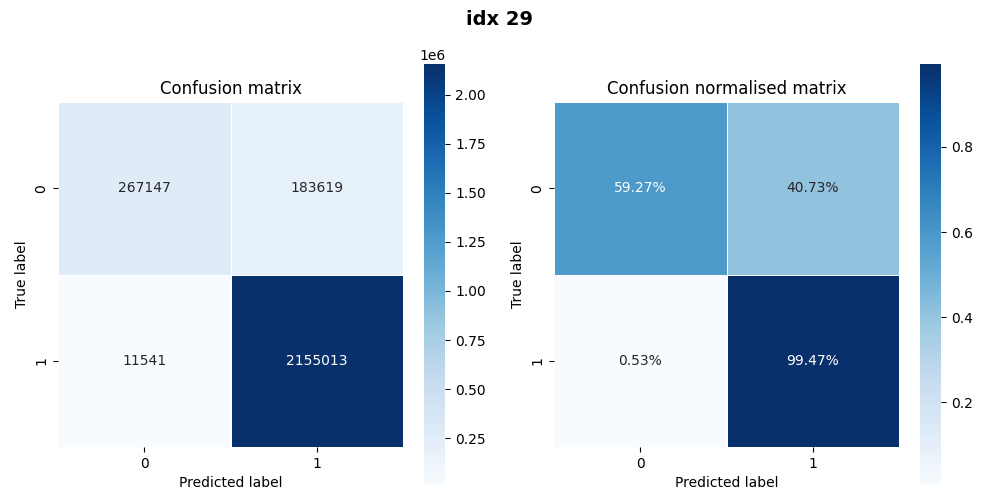
\includegraphics[scale=0.6, cframe=bluepoli 2pt]{./resources/A1_conf_matr_29.png}
 \caption[A1 test confusion matrix]
    {Testing confusion matrix of A1 predictions on image n. 29}
\end{figure}

\begin{figure}[H]
 \centering
 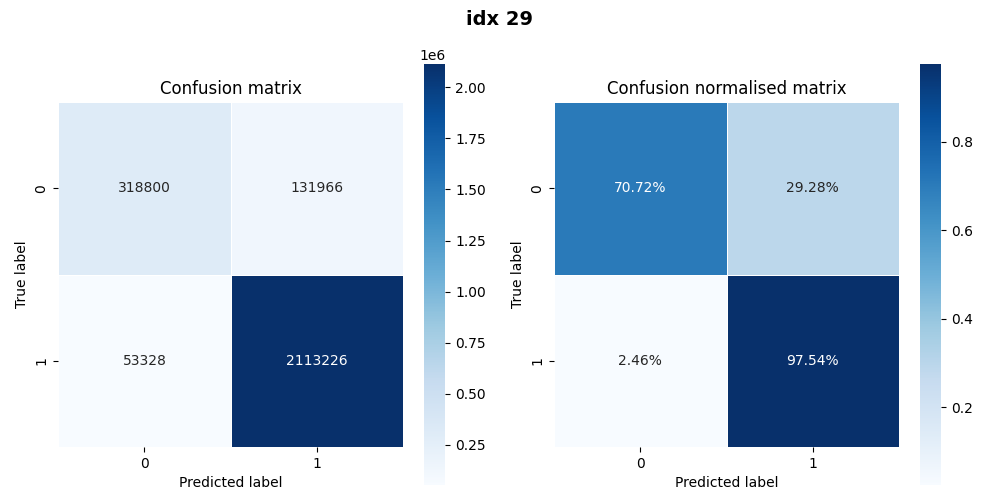
\includegraphics[scale=0.6, cframe=bluepoli 2pt]{./resources/I2_conf_matr_29.png}
 \caption[I2 test confusion matrix]
    {Testing confusion matrix of I2 prediction on image n. 29}
\end{figure}

As expected, in the context of this testing results, we can notice that the \textbf{two models behaved quite similarly} and that \textbf{I2 had a certain advantage in terms of prediction balance}. However, I2 performed slightly better, achieving marginally better scores in all indicators except sensitivity. Overall, the two models proved to deliver respectable and sufficiently reliable performances.

\subsection{Testing Visualisations}

\par
In this section, to conclude the testing procedure, we illustrate some of the visual artifact that allow us to judge by eye the behaviour of the two models.

\par
The prediction procedure on the testing image performed by the models produced the following binary probability mask:

\begin{figure}[H]
 \centering
 
\includegraphics[scale=0.2, cframe=bluepoli 2pt]{./resources/A1_avg_29.png}
 \caption[A1 test prediction]
    {Testing prediction performed by A1 on image n. 29}
\end{figure}

\begin{figure}[H]
 \centering
 
\includegraphics[scale=0.2, cframe=bluepoli 2pt]{./resources/I2_avg_29.png}
 \caption[A1 test prediction]
    {Testing prediction performed by I2 on image n. 29}
\end{figure}

\par
The mask, filtered to a threshold of 0.5, delivers our segmentation prediction:

\begin{figure}[H]
 \centering
 
\includegraphics[scale=0.2, cframe=bluepoli 2pt]{./resources/A1_pred_image_29.png}
 \caption[A1 thresholded test prediction]
    {Testing thresholded prediction performed by A1 on image n. 29}
\end{figure}

\begin{figure}[H]
 \centering
 
\includegraphics[scale=0.2, cframe=bluepoli 2pt]{./resources/I2_pred_image_29.png}
 \caption[I2 thresholded test prediction]
    {Testing thresholded  prediction performed by I2 on image n. 29}
\end{figure}

The following image shows a visual comparison between the predictions and the true segmentation mask available in the dataset, where:

\begin{itemize}
    \item White pixels are correct positive classifications.
    \item Black pixels are correct negative classifications.
    \item Green pixels are false positive classifications (Type 1 error).
    \item Red pixels are false positive classifications (Type 2 error).
\end{itemize}

\begin{figure}[H]
 \centering
 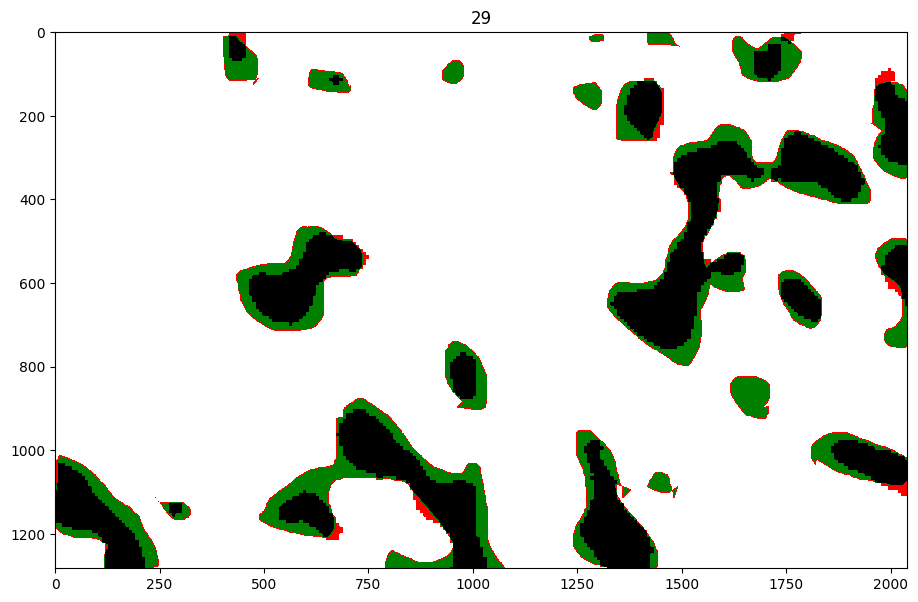
\includegraphics[scale=0.6]{./resources/A1_comp_29.png}
 \caption[A1 test prediction comparison]
    {Visual comparison of prediction performed by A1 on image n. 29 with true mask}
\end{figure}

\begin{figure}[H]
 \centering
 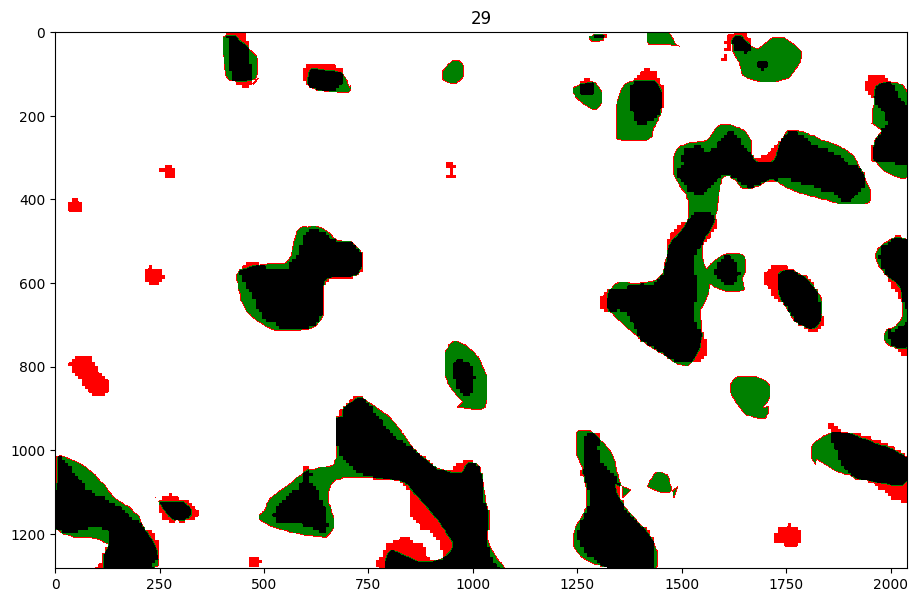
\includegraphics[scale=0.6]{./resources/I2_comp_29.png}
 \caption[I2 test prediction comparison]
    {Visual comparison of prediction performed by I2 on image n. 29 with true mask}
\end{figure}

\chapter{Conclusions}
\par
In conclusion, our replication has been successful, despite the limits in the availability of the original data and the computational resources constrains. This shows that identification of tumor cells using machine learning with good accuracy is possible. Looking ahead, continued improvements in machine learning and data collection show great potential for enhancing accuracy in tumor classification.

%-------------------------------------------------------------------------
%	APPENDICES
%-------------------------------------------------------------------------

\cleardoublepage
\addtocontents{toc}{\vspace{2em}} % Add a gap in the Contents, for aesthetics

% LIST OF FIGURES
\listoffigures

% LIST OF TABLES
\listoftables

\cleardoublepage

\end{document}